\documentclass[graphics]{beamer}
\usepackage[english]{babel}
\usepackage[utf8]{inputenc}
\usepackage{tcolorbox}
\usepackage{pgfpages}
\usepackage{hyperref}

\setbeameroption{show notes}
\setbeameroption{show notes on second screen=right}

\usetheme{ENSLyon}

\title[Title]{Dicotomix}
\author[T.S]{M. Guy, E. Hazard, E. Kerinec, F. Lecuyer, P. Mangold,\\ A. Martin, R. Pellerin, N. Pinson, A. Slowik, T. Stérin}
\date{\today}

\setbeamersize{text margin left=20pt,text margin right=20pt}
\setbeamertemplate{navigation symbols}{}
\usecolortheme{ENSLyon_blue}
\addtobeamertemplate{navigation symbols}{}{
	\usebeamerfont{footline}
	\usebeamercolor[fg]{footline}
	\hspace{1em}
	\insertframenumber/\inserttotalframenumber
}

\begin{document}

\begin{frame}
	\titlepage
	\begin{center}
		
\includegraphics[scale=0.2]{dicotomix}
		
\includegraphics[scale=0.08]{logoens}
		\hspace{2em}
		
\includegraphics[scale=0.55]{ars}
		\hspace{2em}
		
\includegraphics[scale=0.3]{hospices_civils_de_lyon}
	\end{center}
\end{frame}

\begin{frame}{Some figures about Dicotomix}
	\begin{itemize}
		\item 24 contributors
		\item 300 commits
		\item 50 hours meeting at ENS
		\item 30 hours meeting outside
		\item 2 hackathons
	\end{itemize}
\end{frame}

\section*{Content}
\begin{frame}
	\tableofcontents
\end{frame}

\section{Introduction}
\subsection{Motivations}

\begin{frame}{Charcot disease and locked-in syndrome}
	\begin{center}
		\begin{itemize}
			\item Almost entirely paralized
			\item Keeping all cognitive abilities
		\end{itemize}
	\end{center}
\end{frame}

\subsection{Approach}

\newcommand{\background}[5]{%
	\begin{pgfonlayer}{background}
		% Left-top corner of the background rectangle
		\path (#4.west |- #1.north)+(-0.25,0.5) node (a1) {};
		% Right-bottom corner of the background rectanle
		\path (#2.east |- #3.south)+(+0.25,-0.25) node (a2) {};
		\path[fill=yellow!20,rounded corners, draw=black!50,dashed,thick]
		(a1) rectangle (a2);% Draw the background
		\path (a1.east |- a1.south)+(1.5,-.1) node (u1)[]
		{\scriptsize\textit{#5}};
	\end{pgfonlayer}}
	
\begin{frame}{First, get in touch with people}
	\begin{center}
		\vspace{-0.8cm}
		\hspace{-1cm}
		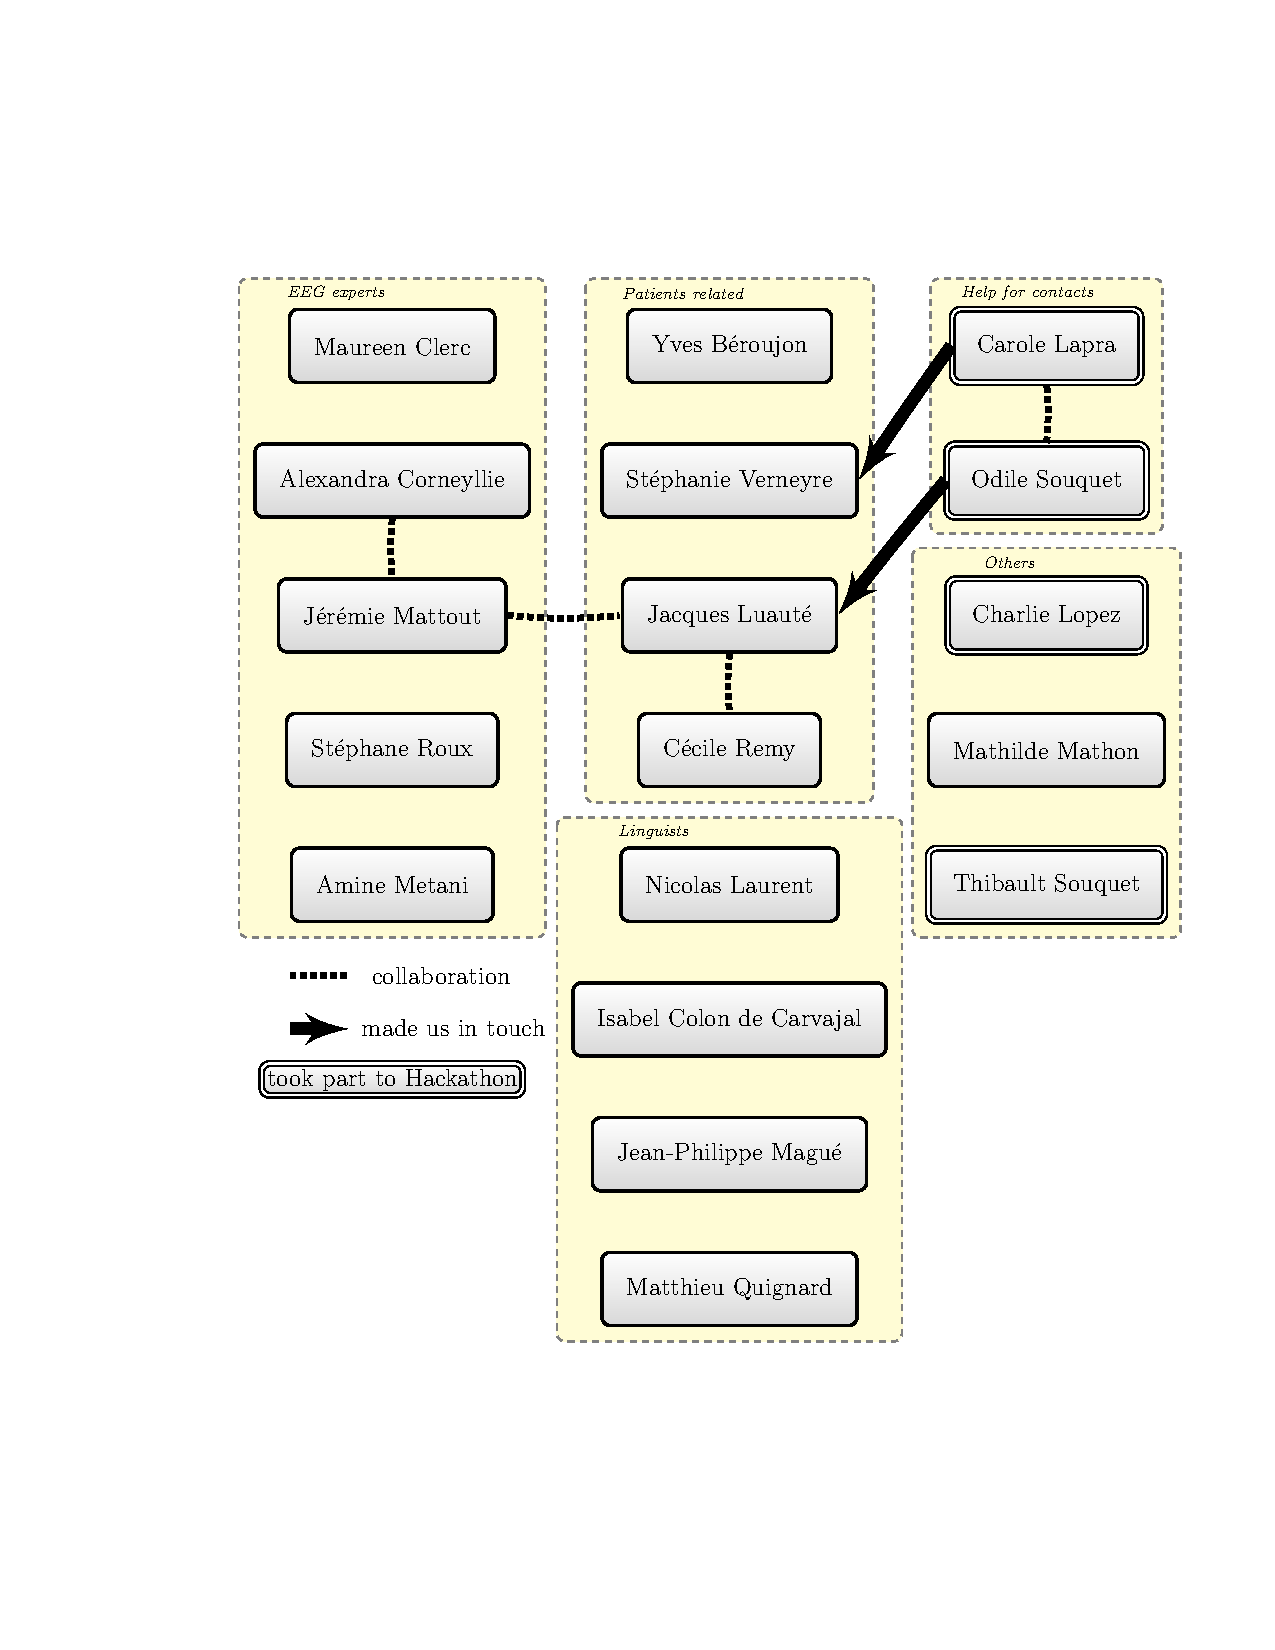
\includegraphics[scale=0.3]{graphe_intervenants.pdf}
	\end{center}
\end{frame}

\begin{frame}{BCI (Brain Computer Interface)}
	\begin{center}
		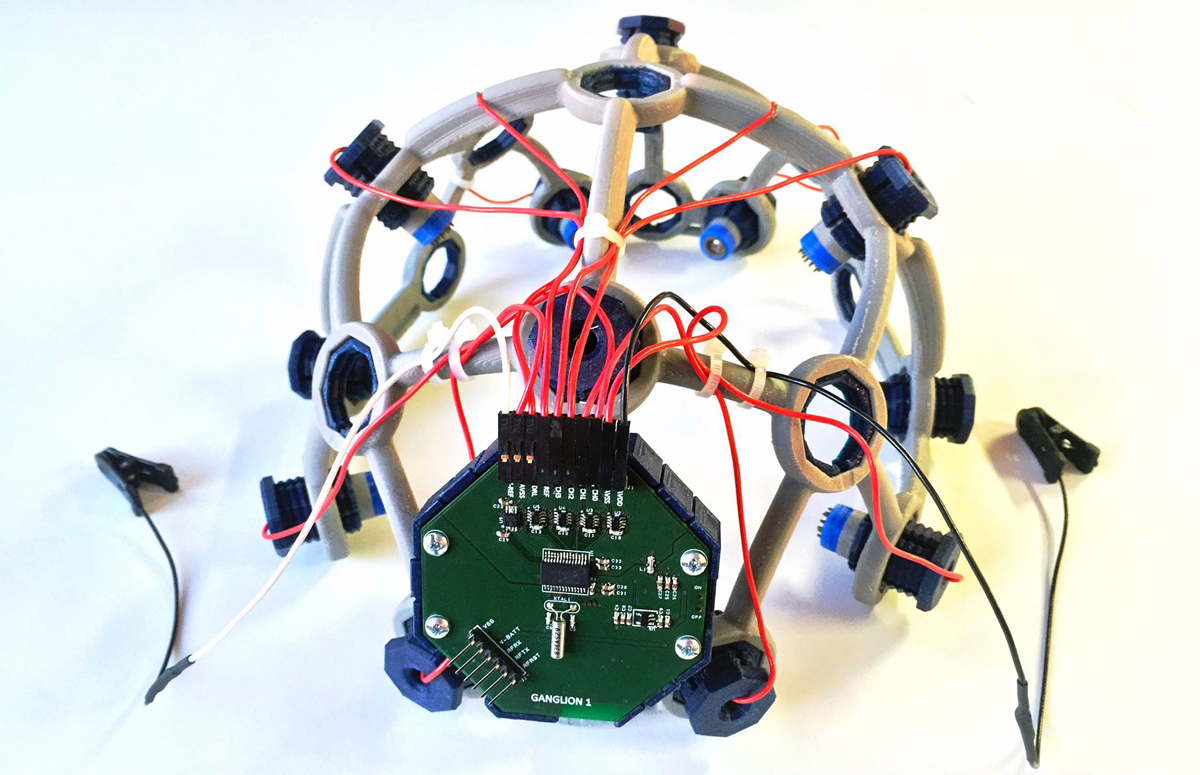
\includegraphics[scale=0.1]{bci}
		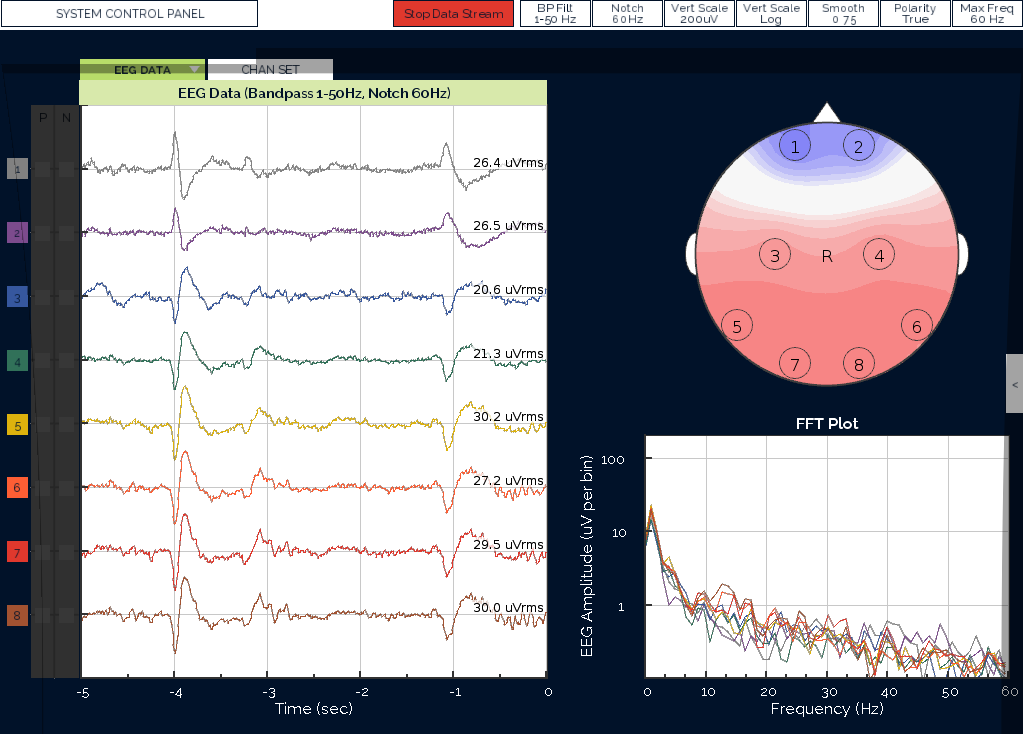
\includegraphics[scale=0.1]{openbci}
	\end{center}
	\begin{center}
		\begin{tcolorbox}[colback=green!5,colframe=green!40!black,title=Initial Idea]
			Use of BCI for people who cannot move anything.
			\note{This was our initial idea.}
		\end{tcolorbox}
		\pause
		\begin{tcolorbox}[colback=red!5,colframe=red!40!black,title=Reallity]
			Problem is having a good signal and then dealing with it was very hard!
			\note{We decided to make a break with BCI and to focus on the software part. But we are currently working on it again with Stephan Roux and Amine Metani (physicians at ENS Lyon).}
		\end{tcolorbox}
		\note{Talk about the first meeting with Luauté who tells us to stop working on BCI...}
	\end{center}
\end{frame}

\begin{frame}{Existing methods : EJASINT}
	\begin{center}
		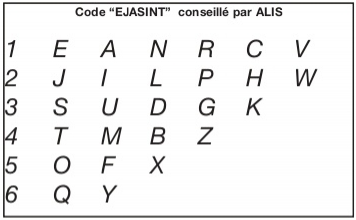
\includegraphics[scale=0.7]{ejasint}
	\end{center}
\end{frame}

\begin{frame}{Existing methods : ARS}
	\begin{center}
		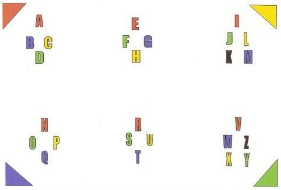
\includegraphics[scale=0.9]{tableau_lettres_transparent}
	\end{center}
\end{frame}

\begin{frame}{Existing methods : "Par-Lé-Si-Lab"}
	\begin{center}
		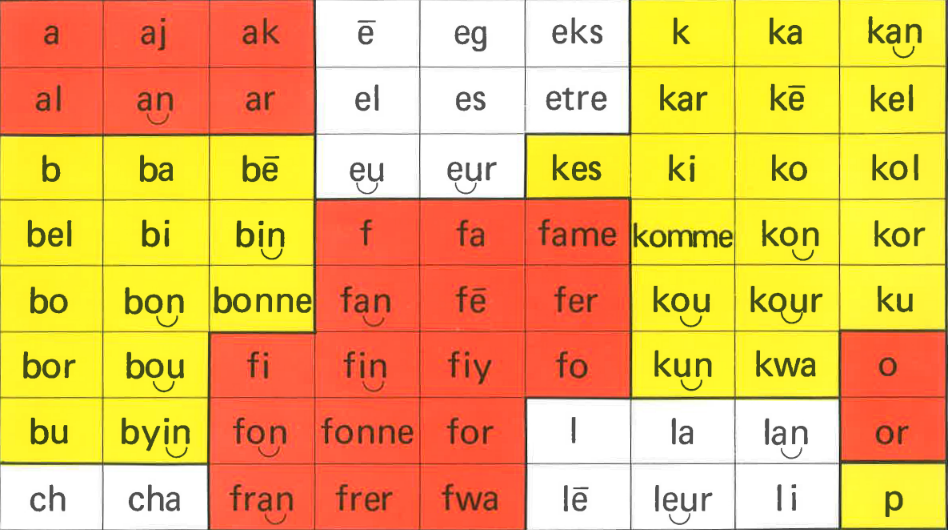
\includegraphics[scale=0.3]{parler_syllabes}
	\end{center}
\end{frame}

\section{The Dicotomix's original approach}
\subsection{The concept}

\begin{frame}{Concept}
	\begin{center}
		\begin{itemize}
			\item Writing word by word rather than spelling (reduce frustration)
			\item Optimizing each question
				\note[item]{First, we thought about using something like "Akinator".}
			\item Making it intuitive thanks to a simple interface
				\note[item]{We've worked with designers.}
			\item The only requirement is a binary input
				\note[item]{Our software is indenpent of the binary input.}
		\end{itemize}
	\end{center}
\end{frame}

\begin{frame}{Demo}
	\begin{center}
		
\includegraphics[scale=0.6]{aladdin}
	\end{center}
\end{frame}

\subsection{Algorithm}

\begin{frame}{Algorithm}
	\begin{center}
		\begin{itemize}
			\item Dichotomy over a dictionary (right/left signals)
			\item Frequencies of words taken into account
				\note[item]{Explainations on the board!}
			\item We can deduce the prefix which is certain and mark it green.
				\note[item]{This is espacially useful for error detection. We'll see later.}
		\end{itemize}
	\end{center}
\end{frame}

\begin{frame}{The proof that Dicotomix is fast!}
	\begin{center}
		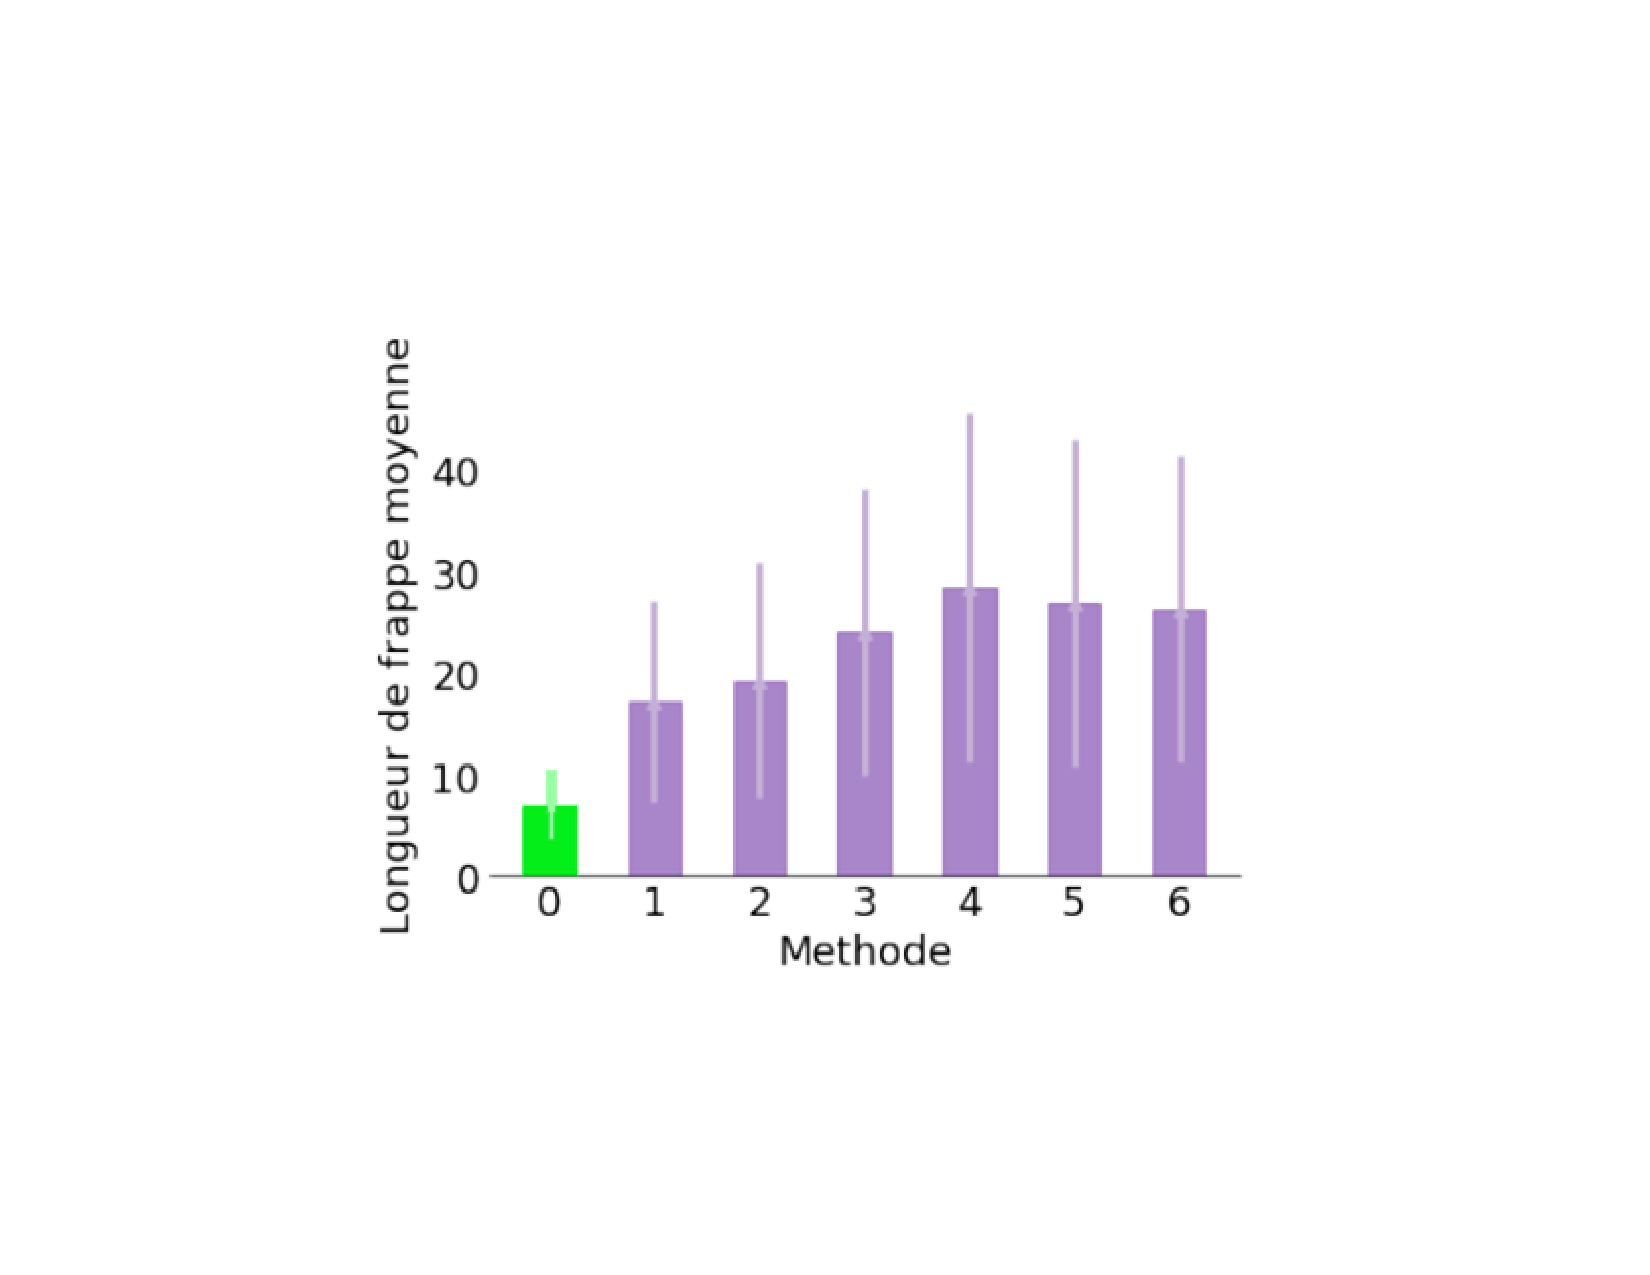
\includegraphics[scale=0.35]{graphe_comparatif.pdf}
	\end{center}
\end{frame}

\begin{frame}{Assets / Drawbacks}
	\begin{tcolorbox}[colback=green!5,colframe=green!40!black,title=Assets]
		\begin{itemize}
			\item Faster than spelling
				\note[item]{We made a comparison between some existing methods and ours. This could also be proved theoretically.}
			\item One can get better by training
				\note[item]{This will be confirmed by the study.}
			\item Could even have some fun playing with Dicotomix!
				\note[item]{The user is not as passive as in the methods described before.}
		\end{itemize}
	\end{tcolorbox}
	\pause
	\begin{tcolorbox}[colback=red!5,colframe=red!40!black,title=Drawbacks]
		\begin{itemize}
			\item It's hard to deal with mistakes
			\item Counter intuitive at the beginning (requires some training)
			\item Requires to be really focused
			\item What about proper names ?
		\end{itemize}
	\end{tcolorbox}
\end{frame}

\begin{frame}{How to deal with mistakes ?}
	\begin{itemize}
		\item Cannot automatically correct mistakes
			\note[item]{What is the patient is wrong on the first letter ?}
		\pause
		\item How to discard last choice ?
			\note[item]{We've implemented it, we will show you next.}
		\pause
		\item How to edit the current sentence ?
			\note[item]{Currently, Dicotomix aimed to be used in everyday life, not for writing a book!}
		\pause
		\item Can we deal with semantic mistakes ?
	\end{itemize}
\end{frame}

\begin{frame}{Demo (strikes back!)}
	\begin{center}
		
\includegraphics[scale=0.6]{aladdin2}
	\end{center}
\end{frame}

\begin{frame}{Modularity}
	\begin{center}
		\begin{itemize}
			\item Use of every possible dictionary %ajout de mots
			\item Possibility to change frequencies using some heuristics
			\item Adaptation to the patient
		\end{itemize}
	\end{center}
\end{frame}



\begin{frame}{The ergonomy of Dicotomix}
	\begin{center}
		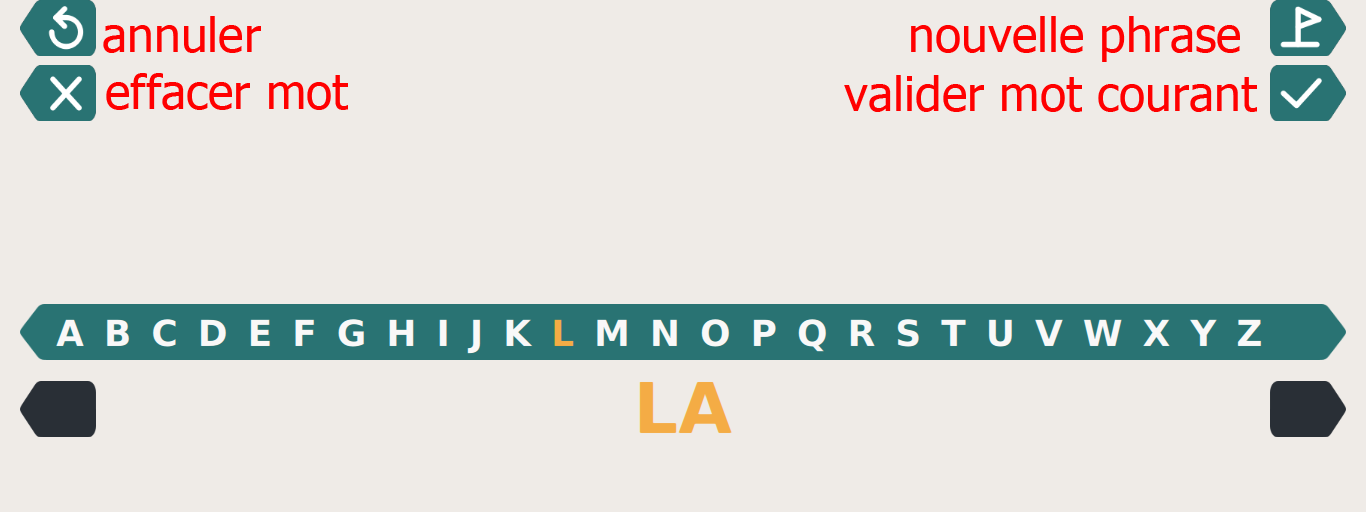
\includegraphics[scale=0.2]{vierge}
	\end{center}
\end{frame}

\begin{frame}{The ergonomy of Dicotomix 2}
	\begin{center}
		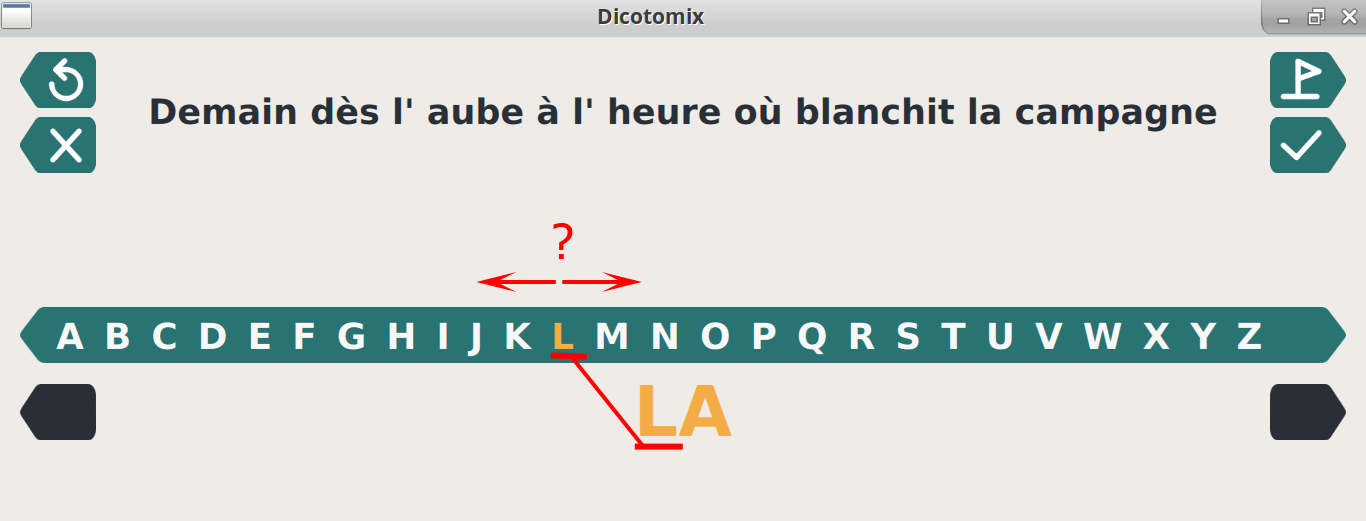
\includegraphics[scale=0.2]{example1}
	\end{center}
\end{frame}

\begin{frame}{The ergonomy of Dicotomix 3}
	\begin{center}
		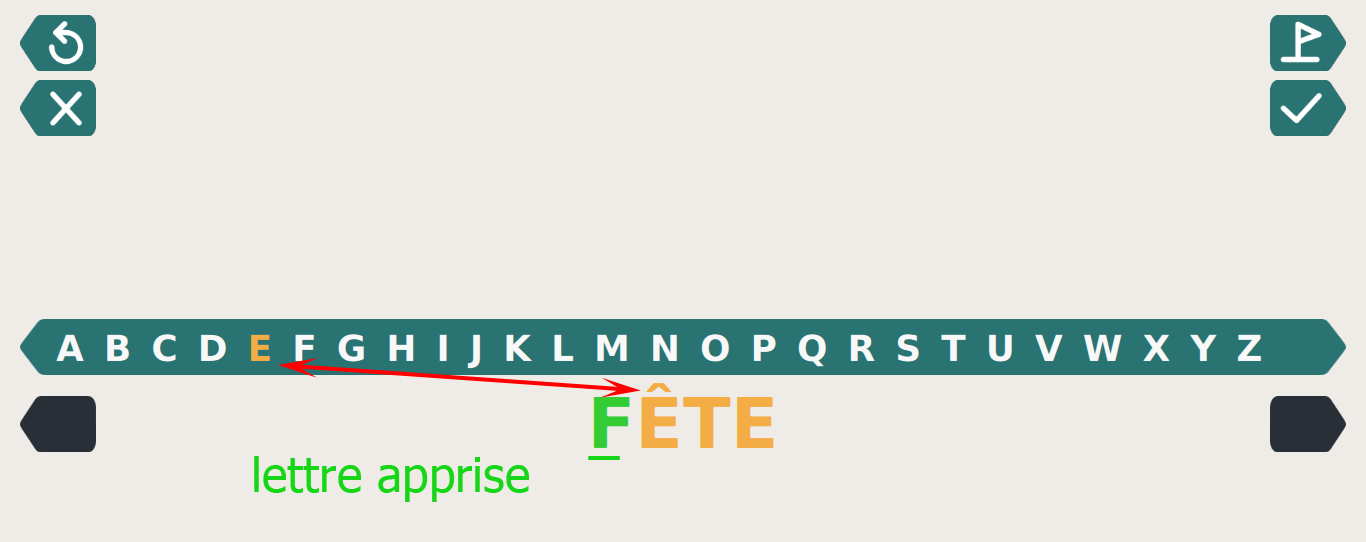
\includegraphics[scale=0.2]{encours}
	\end{center}
\end{frame}

\section{What's next ?}
\subsection{Test phase}
\begin{frame}{Clinical trials}
	\begin{center}
		\begin{itemize}
			\item Hôpital Lyon Nord %à vérifier
			\item a few patients
			\item a training phase and a evaluation phase %décrire le protocole
		\end{itemize}
	\end{center}
\end{frame}


\begin{frame}{Test protocol}
	A training session:
	\begin{itemize}
		\item 10 words to find using Dicotomix
		\item Spell a name
		\item 3 questions
		\item Chatting ("Do you want to say anything?")
	\end{itemize}
	Evaluation: write a text using Dicotomix, then the usual method
\end{frame}

\subsection{Distribution}
\begin{frame}{Reaching patients}
	\hspace{7cm}
	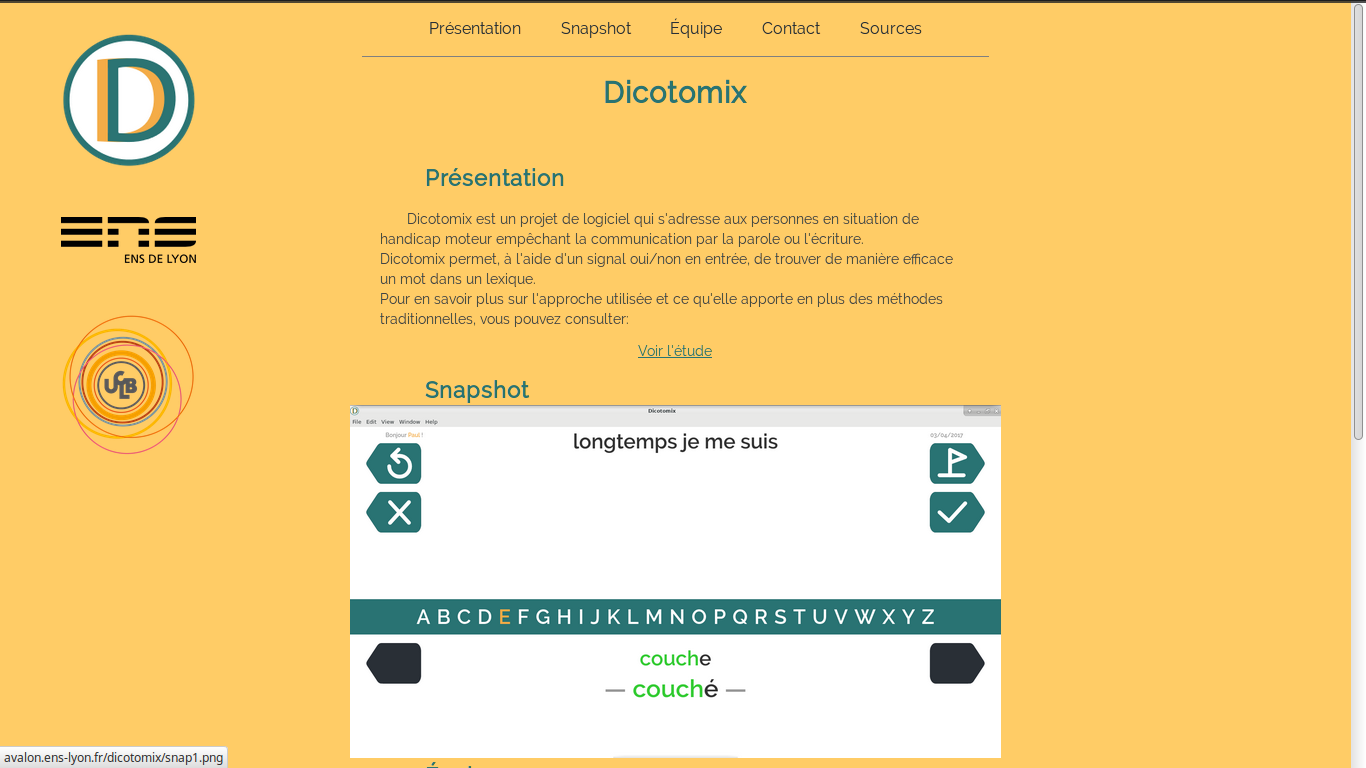
\includegraphics[scale=0.075]{website}\\
	\begin{itemize}
		\item Help of metropole de Lyon and ARSLA
			\note[item]{With possibily other partners...}
		\pause
		\item The code is available from our website : \hyperref[http://avalon.ens-lyon.fr/dicotomix]{http://avalon.ens-lyon.fr/dicotomix}
		\pause
		\item As well as on GitHub
		\pause
		\item A Tutorial is available
	\end{itemize}
	\hspace{10cm}
	
\includegraphics[scale=0.07]{opensource}
\end{frame}

\begin{frame}{Questions ?}
	\begin{center}
		Thank you for your attention!
		\begin{center}
			\begin{picture}(100,100)
				\put(15,30){
\includegraphics[scale=0.2]{dicotomix}}
				\put(-15,50){
\includegraphics[scale=0.2]{ars}}
				\put(55,-25){
\includegraphics[scale=0.1]{alis}}
				\put(90,30){
\includegraphics[scale=0.1]{arsla}}
				\put(30,80){
\includegraphics[scale=0.05]{logoens}}
				\put(-15,0){
\includegraphics[scale=0.2]{hospices_civils_de_lyon}}
			\end{picture}
		\end{center}
		\vspace{1cm}
		Special thanks to all our contacts!
	\end{center}
\end{frame}
\end{document}
